\documentclass[11pt]{amsart}

\usepackage[utf8]{inputenc}
\usepackage[T1]{fontenc}
\usepackage{lmodern}
\usepackage{amsmath,amssymb,amsthm,mathtools}
\usepackage{microtype}
\usepackage{xcolor}
\usepackage{booktabs}
\usepackage{array}
\usepackage{enumitem}
\usepackage{tikz}
\usepackage{float}
\usepackage[margin=1.15in]{geometry}
\usepackage[colorlinks=true,linkcolor=blue!50!black,citecolor=green!40!black,urlcolor=blue!50!black]{hyperref}
\usepackage[capitalize,nameinlink]{cleveref}

\newtheorem{theorem}{Theorem}[section]
\newtheorem{proposition}[theorem]{Proposition}
\newtheorem{lemma}[theorem]{Lemma}
\newtheorem{corollary}[theorem]{Corollary}
\newtheorem{conjecture}[theorem]{Conjecture}
\theoremstyle{definition}
\newtheorem{definition}[theorem]{Definition}
\newtheorem{remark}[theorem]{Remark}
\newtheorem{problem}[theorem]{Problem}
\crefname{problem}{Problem}{Problems}
\crefname{conjecture}{Conjecture}{Conjectures}

\raggedbottom
\newcommand{\Z}{\mathbb{Z}}
\newcommand{\eps}{\varepsilon}
\newcommand{\LEAN}{\textsc{Lean}}
\newcommand{\lean}[1]{\texttt{#1}}
\newcommand{\up}{\texttt{+}}
\newcommand{\dn}{\texttt{-}}

\title{Recam\'an's sequence at high altitude}

\author{Cl\'ement Chardine}

\subjclass[2020]{11B83; 37B10, 68V15}
\keywords{Recam\'an's sequence, OEIS A005132, growth of integer sequences, self-interacting walks, subadditivity, Lean}

\begin{document}

\begin{abstract}
Recam\'an's sequence starts at $0$, and its $n$th step subtracts $n$ if the result is non-negative and new, and adds $n$
otherwise. The only published upper bound on its growth appears to be the trivial $a(n)\le n(n+1)/2$. We show that, far above
the values it has visited, the sequence follows a rule with no arithmetic in it: a $\pm1$ walk steps up exactly when some earlier
stretch of it has a prescribed mean. This reduces the growth question to a game on $\pm1$ walks. A one-page argument then gives
$\limsup a(n)/n^2\le3/26$, and a small verified search gives $1/14$. We then study the game itself. If its reach rate is positive,
optimal plays converge to stationary walks that obey the rule at every step, with no opponent. Every inequality $W\le cD$, where $W$
counts the up-steps of a $\pm1$ word that satisfy the rule's condition and $D$ counts its down-steps, gives
$\limsup a(n)/n^2\le(c-1)/(2c+2)$. We prove it for $c=2$. The case $c=1$, which we state as a conjecture, would give
$a(n)=o(n^2)$, and we show that this is equivalent to subtractions having frequency $1/2$. We also describe the natural approaches
to the conjecture that fail, with the words that refute them. The bounds on the sequence, the reduction to the game and the
consequences of $W\le cD$ are formalized in Lean~4, in about $1200$ lines.
\end{abstract}

\maketitle

\begin{flushright}
\small\emph{What goes up must come down.}\\ Proverb (for our purposes, a conjecture)
\end{flushright}

\section{Introduction}

\subsection{The walk}
Start at $0$, and take steps of length $1$, then $2$, then $3$, and so on. Always step back if you can; but never below $0$, and never
back to a place you have already been. If you cannot step back, step forward.

From $0$ we cannot step back by $1$, so we go to $1$. We cannot step back by $2$, so we go to $3$; and then, since $3-3=0$ has been
visited, to $6$. Now $6-4=2$ is new, and we go there. Continuing,
\[
  0,\ 1,\ 3,\ 6,\ 2,\ 7,\ 13,\ 20,\ 12,\ 21,\ 11,\ 22,\ 10,\ 23,\ 9,\ 24,\ 8,\ 25,\ 43,\ 62,\ 42,\ 63,\ 41,\ 18,\ \dots
\]
This is Recam\'an's sequence, A005132 in the OEIS \cite{OEIS}. Formally, $a(0)=0$, and
\begin{equation}\label{eq:def}
  a(n)=\begin{cases}
    a(n-1)-n & \text{if } a(n-1)-n\ge 0 \text{ and } a(n-1)-n\notin\{a(0),\dots,a(n-1)\},\\
    a(n-1)+n & \text{otherwise.}
  \end{cases}
\end{equation}
Bernardo Recam\'an Santos sent it to Neil Sloane in 1991 \cite{Recaman1991}, and it has been popular ever since
\cite{Sloane1999,Cousins2022,Sloane2023}. The best known question about it is whether every number appears. After more than $10^{612}$ terms, the
smallest absentee is $852655$ \cite{OEIS,Chaffin2026}. This paper will not find it.

\begin{figure}[H]
\centering
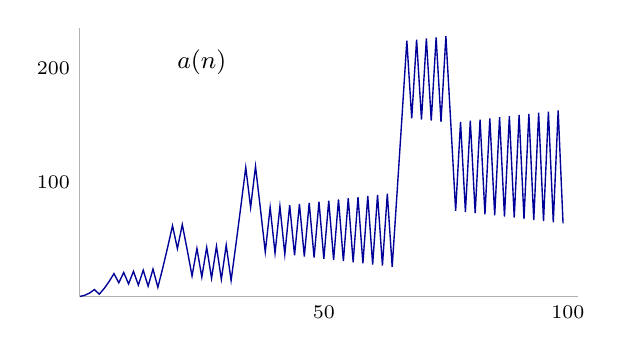
\begin{tikzpicture}[x=0.062cm,y=0.0145cm]
\draw[gray!60] (0,0)--(102,0); \draw[gray!60] (0,0)--(0,235);
\foreach \x in {50,100} \node[below,font=\scriptsize] at (\x,0) {$\x$};
\foreach \y in {100,200} \node[left,font=\scriptsize] at (0,\y) {$\y$};
\draw[blue!60!black,line width=0.5pt] plot coordinates {(0,0)(1,1)(2,3)(3,6)(4,2)(5,7)(6,13)(7,20)(8,12)(9,21)(10,11)(11,22)(12,10)(13,23)(14,9)(15,24)(16,8)(17,25)(18,43)(19,62)(20,42)(21,63)(22,41)(23,18)(24,42)(25,17)(26,43)(27,16)(28,44)(29,15)(30,45)(31,14)(32,46)(33,79)(34,113)(35,78)(36,114)(37,77)(38,39)(39,78)(40,38)(41,79)(42,37)(43,80)(44,36)(45,81)(46,35)(47,82)(48,34)(49,83)(50,33)(51,84)(52,32)(53,85)(54,31)(55,86)(56,30)(57,87)(58,29)(59,88)(60,28)(61,89)(62,27)(63,90)(64,26)(65,91)(66,157)(67,224)(68,156)(69,225)(70,155)(71,226)(72,154)(73,227)(74,153)(75,228)(76,152)(77,75)(78,153)(79,74)(80,154)(81,73)(82,155)(83,72)(84,156)(85,71)(86,157)(87,70)(88,158)(89,69)(90,159)(91,68)(92,160)(93,67)(94,161)(95,66)(96,162)(97,65)(98,163)(99,64)};
\node[font=\small] at (25,205) {$a(n)$};
\end{tikzpicture}\hspace{0.9cm}
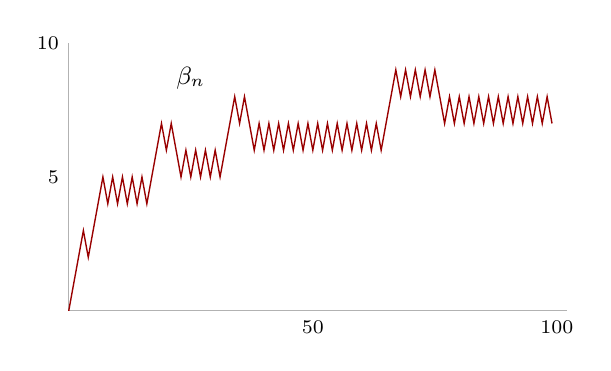
\begin{tikzpicture}[x=0.062cm,y=0.34cm]
\draw[gray!60] (0,0)--(102,0); \draw[gray!60] (0,0)--(0,10);
\foreach \x in {50,100} \node[below,font=\scriptsize] at (\x,0) {$\x$};
\foreach \y in {5,10} \node[left,font=\scriptsize] at (0,\y) {$\y$};
\draw[red!60!black,line width=0.5pt] plot coordinates {(0,0)(1,1)(2,2)(3,3)(4,2)(5,3)(6,4)(7,5)(8,4)(9,5)(10,4)(11,5)(12,4)(13,5)(14,4)(15,5)(16,4)(17,5)(18,6)(19,7)(20,6)(21,7)(22,6)(23,5)(24,6)(25,5)(26,6)(27,5)(28,6)(29,5)(30,6)(31,5)(32,6)(33,7)(34,8)(35,7)(36,8)(37,7)(38,6)(39,7)(40,6)(41,7)(42,6)(43,7)(44,6)(45,7)(46,6)(47,7)(48,6)(49,7)(50,6)(51,7)(52,6)(53,7)(54,6)(55,7)(56,6)(57,7)(58,6)(59,7)(60,6)(61,7)(62,6)(63,7)(64,6)(65,7)(66,8)(67,9)(68,8)(69,9)(70,8)(71,9)(72,8)(73,9)(74,8)(75,9)(76,8)(77,7)(78,8)(79,7)(80,8)(81,7)(82,8)(83,7)(84,8)(85,7)(86,8)(87,7)(88,8)(89,7)(90,8)(91,7)(92,8)(93,7)(94,8)(95,7)(96,8)(97,7)(98,8)(99,7)};
\node[font=\small] at (25,8.7) {$\beta_n$};
\end{tikzpicture}
\caption{The first hundred terms (left), and their balance $\beta_n$, additions minus subtractions (right). The left
picture is the familiar one; this paper is about the right one.}
\label{fig:balance}
\end{figure}

\subsection{The question}
How fast does it grow? Since the $n$th step has length $n$,
\begin{equation}\label{eq:trivial}
  a(n)\le 1+2+\dots+n=\frac{n(n+1)}2 ,
\end{equation}
with equality if one never steps back. We have found no better upper bound in the literature. In fact the sequence steps back
about half of the time: among the first hundred million steps, additions outnumber subtractions by only $32$, and $a(n)\le7.78\,n$
in that range. Eppstein \cite{Eppstein2019} fits such data with growth of order $n\log n$, but does not find them clear enough to
settle the rate.

The natural way to improve \eqref{eq:trivial} is to show that a few consecutive steps cannot all be additions. This improves the
constant, but each improvement needs more cases than the last. In this paper we look at long stretches of steps at once, through a
game, and we isolate the one inequality on words that this approach lacks.

\subsection{What we prove}
Let $S(N)$ be the number of subtractions among the first $N$ steps.

\begin{theorem}\label{thm:main}
The following hold.
\begin{enumerate}[label=\textup{(\alph*)}]
  \item $\limsup a(N)/N^2\le 3/26$.
  \item $\limsup a(N)/N^2\le 1/14$.
  \item $S(N)\le N/2$ for every $N$, and $\liminf S(N)/N\ge 3/7$.
\end{enumerate}
\end{theorem}

Part (a) has a proof of about a page, without computation. Part (b) implies (a); its proof asks the Lean kernel to examine
about $80\,000$ positions, which takes half a minute. Part (c) says that additions lead subtractions by at most $N/7+o(N)$. At
$N=10^8$ this allows a lead of some fourteen million, and the actual lead is $32$.

So the constants are far from the truth, and they are not the main content of the paper. Each is an upper bound $R(L)/L$ for a
quantity $\rho\in[0,\frac17]$, the \emph{reach rate} of a game, which satisfies $\limsup a(N)/N^2\le\rho/2$. If $\rho=0$, the
method gives $a(N)=o(N^2)$; if $\rho>0$, it gives a positive constant and no more. We reformulate the question whether $\rho=0$
several times:
\begin{center}
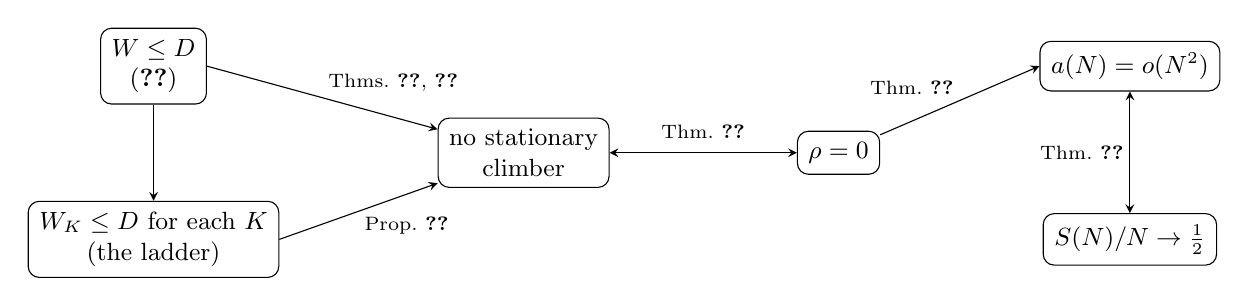
\begin{tikzpicture}[>=stealth,every node/.style={align=center,font=\small,inner sep=4pt},box/.style={draw,rounded corners},
 lab/.style={font=\scriptsize,inner sep=2pt}]
\node[box] (D) at (0,0) {$W\le D$\\ (\cref{conj:wd})};
\node[box] (K) at (0,-2.2) {$W_K\le D$ for each $K$\\ (the ladder)};
\node[box] (C) at (4.7,-1.1) {no stationary\\ climber};
\node[box] (R) at (8.7,-1.1) {$\rho=0$};
\node[box] (A) at (12.4,0) {$a(N)=o(N^2)$};
\node[box] (F) at (12.4,-2.2) {$S(N)/N\to\frac12$};
\draw[->] (D) -- (K);
\draw[->] (K.east) -- (C) node[midway,lab,below right] {Prop.~\ref{prop:ladder}};
\draw[->] (D.east) -- (C) node[midway,lab,above right] {Thms.~\ref{thm:dial}, \ref{thm:climber}};
\draw[<->] (C) -- (R) node[midway,lab,above=3pt] {Thm.~\ref{thm:climber}};
\draw[->] (R) -- (A.west) node[midway,lab,above left] {Thm.~\ref{thm:growth}};
\draw[<->] (A) -- (F) node[midway,lab,left] {Thm.~\ref{thm:frequency}};
\end{tikzpicture}
\end{center}
From right to left: \cref{thm:growth} replaces the sequence by a game with no arithmetic in it, \cref{thm:climber} replaces the
optimal plays of the game by stationary walks with no opponent, and \cref{thm:dial} (or the ladder, \cref{prop:ladder})
reduces the question to an inequality $W\le D$ between two counts on finite words (\cref{sec:dial}). The inequality is easy to test on any given word, and we cannot prove it.

\subsection{How to read this paper}
Sections \ref{sec:balance}--\ref{sec:values} prove \cref{thm:main}. Sections \ref{sec:climbers} and \ref{sec:dial} contain the ideas that we expect to be most useful elsewhere; a reader who likes combinatorics on words may start at
\cref{sec:dial} and needs only \cref{def:game}. \Cref{sec:obstructions} lists ideas that fail, and \cref{sec:problems} lists problems.

A \emph{walk} is a function $u:\Z_{\ge0}\to\Z$ with $u_{t+1}=u_t\pm1$. \emph{Step $t$} goes from $u_t$ to $u_{t+1}$. A \emph{word} is a finite string of signs $\up$ and $\dn$,
identified with the walk from $0$ that it describes. Statements whose heading says \LEAN{} are formalized, and \cref{app:lean} says where. The others
(\cref{thm:climber} and \cref{prop:slack,prop:ladder,prop:convex}) are proved here only, and claims about explicit words are verified
by \lean{tools/check.py}. Statements called
\emph{measured} are outputs of \lean{tools/game.c}; no proof uses them.

\section{One identity, read twice}\label{sec:balance}

Let the \emph{balance} $\beta_n$ be the number of additions minus the number of subtractions among steps $1,\dots,n$; so $\beta_0=0$ and $\beta_n=n-2S(n)$. It is a
walk (\cref{fig:balance}), and by the next lemma it determines the sequence.

\begin{lemma}[The master identity; \LEAN]\label{lem:master}
For $k\le m$,
\begin{equation}\label{eq:master}
  a(m)-a(k)\;=\;m\,(\beta_m-\beta_k)\;-\sum_{k\le i<m}(\beta_i-\beta_k).
\end{equation}
\end{lemma}

\begin{proof}
Both sides vanish for $m=k$. When $m$ increases by one, the left side changes by ${(m+1)(\beta_{m+1}-\beta_m)}$, and so does the right side:
\[
 (m+1)(\beta_{m+1}-\beta_k)-m(\beta_m-\beta_k)-(\beta_m-\beta_k)=(m+1)(\beta_{m+1}-\beta_m). \qedhere
\]
\end{proof}

With $k=0$ it says that $a(N)/N=\beta_N-\frac1N\sum_{i<N}\beta_i$: the quotient $a(N)/N$ is the amount by which the
balance exceeds its own average over the past. We use \eqref{eq:master} in two ways.

\subsection{First reading: growth and the frequency of subtractions}

\begin{theorem}[\LEAN]\label{thm:frequency}
We have $\beta_N\ge0$ and
\[
  \limsup\frac{a(N)}{N^2}\ \le\ \limsup\frac{\beta_N}{N}\ \le\ 2\limsup\frac{a(N)}{N^2}.
\]
In particular $a(N)=o(N^2)$ if and only if $S(N)/N\to\frac12$.
\end{theorem}

\begin{proof}
The identity can be inverted: for $N\ge1$,
\begin{equation}\label{eq:inverse}
  \beta_N=\frac{a(N)}N+\sum_{1\le j<N}\frac{a(j)}{j(j+1)} .
\end{equation}
Indeed both sides are $1$ at $N=1$, and when $N$ increases by one, the right side changes by $(a(N+1)-a(N))/(N+1)$, that is, by $\pm1$. All its terms
are non-negative. Hence $\beta_N\ge a(N)/N\ge0$, which is the first inequality. If $a(j)\le c'j^2$ for $j\ge N_0$, the
right side is at most $c'N+c'N+O_{N_0}(1)$, which is the second.
\end{proof}

\subsection{Second reading: a rule in layers}
Step $m+1$ would like to go to $a(m)-(m+1)$. By \eqref{eq:master}, this value was visited at time $k<m$ if and only if
\begin{equation}\label{eq:layer}
  \sum_{k\le i<m}(\beta_i-\beta_k)=j\,m-1,\qquad\text{where } j=\beta_m-\beta_k-1 .
\end{equation}
So the sequence can be defined through its balance alone: by \eqref{eq:master} with $k=0$,
$a(m)=m\beta_m-\sum_{i<m}\beta_i$, and the balance steps up if and only if $a(m)\le m$ or \eqref{eq:layer} holds for some $k<m$. We
call $j$ the \emph{layer} of the collision. In layer $0$, the number $m$ disappears from the condition:
\begin{equation}\label{eq:wit}
  \beta_m=\beta_k+1\quad\text{and}\quad\sum_{k\le i<m}(\beta_i-\beta_k)=-1 .
\end{equation}
Only the walk between times $k$ and $m$ enters this condition; the number $m$ itself does not. The other layers need
much more area, which a walk accumulates slowly.

\begin{lemma}[Locality; \LEAN]\label{lem:local}
If $0<d$ and $d^2<k+d$, then the value tested by step $k+d+1$ is $a(k)$ if and only if \eqref{eq:wit} holds with $m=k+d$.
\end{lemma}

\begin{proof}
Let $\Sigma$ be the sum in \eqref{eq:layer}. Its terms are at most $0,1,\dots,d-1$ in absolute value, so $|\Sigma+1|\le d(d-1)/2+1\le d^2$. But if
$j\ne0$ then $|\Sigma+1|=|j|m\ge m>d^2$, a contradiction. So $j=0$.
\end{proof}

So all collisions at distance $d$ with $d^2<m$ are in layer $0$. Collisions with older terms are the only other possibility,
and in the next section we hand them over to an opponent.

\section{The game played at high altitude}\label{sec:game}

\begin{definition}\label{def:game}
In a walk $u$, time $s<t$ \emph{witnesses} step $t$ if
\[
  u_t=u_s+1\qquad\text{and}\qquad\sum_{s\le i<t}(u_i-u_s)=-1 .
\]
A \emph{play} of length $L$ is a walk with $u_0\le0$ in which every step $t<L$ from a height $u_t\ge2$ is \emph{forced}:
it goes up if it has a witness, and down if it has none. Steps from heights $\le1$ are \emph{free}. The \emph{reach} $R(L)$ is the
greatest height that a play of length $L$ attains at a time $t\le L$.
\end{definition}

Adding the term $u_t-u_s=1$ to the sum, we can say the rule in words. \emph{From height $p+1$, go up if you stood at $p$ at some earlier time and your mean height
since then is exactly $p$. Otherwise go down.} Equivalently, the areas above and below $p$ since that time are equal (\cref{fig:play}). There is also a
picture without areas. Put $P_t=(t,\sum_{i<t}u_i)$, so that the slope of the curve $P$ at time $t$ is $u_t$. Time $s$ is a witness if $P_t$ lies exactly one unit below the line through $P_s$ and
$P_{s+1}$, at a moment when the slope has grown by one.

\begin{figure}[H]
\centering
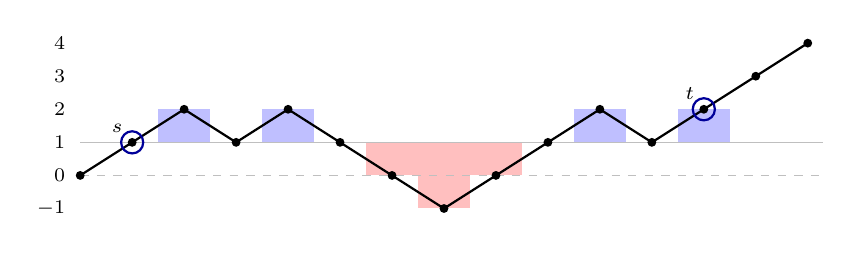
\begin{tikzpicture}[x=0.66cm,y=0.42cm]
\foreach \x/\h in {2/2,4/2,10/2,12/2} {\fill[blue!25] (\x-0.5,1) rectangle (\x+0.5,\h);}
\foreach \x/\h in {6/0,7/-1,8/0} {\fill[red!25] (\x-0.5,1) rectangle (\x+0.5,\h);}
\draw[gray!50] (0,1) -- (14.3,1);
\draw[gray!50,dashed] (0,0) -- (14.3,0);
\foreach \y in {-1,0,1,2,3,4} {\node[left,font=\scriptsize] at (-0.1,\y) {$\y$};}
\draw[thick] (0,0)--(1,1)--(2,2)--(3,1)--(4,2)--(5,1)--(6,0)--(7,-1)--(8,0)--(9,1)--(10,2)--(11,1)--(12,2)--(13,3)--(14,4);
\foreach \x/\y in {0/0,1/1,2/2,3/1,4/2,5/1,6/0,7/-1,8/0,9/1,10/2,11/1,12/2,13/3,14/4} {\fill (\x,\y) circle (1.6pt);}
\draw[thick,blue!60!black] (1,1) circle (4pt) (12,2) circle (4pt);
\node[font=\scriptsize,above left] at (1,1) {$s$};
\node[font=\scriptsize,above left] at (12,2) {$t$};
\end{tikzpicture}
\caption{The fastest way to height $4$ (\cref{thm:four}). The walk goes up at time $t=12$ because at time $s=1$ it stood
one lower, and has since spent as much area above that height (blue) as below it (red).}
\label{fig:play}
\end{figure}

\begin{proposition}[Windows are plays; \LEAN]\label{prop:window}
Let $M(n)=\max_{i\le n}a(i)$. If $n\ge(L+2)^2$, $c\ge0$ is an integer and $M(n)\le a(n)+cn$, then $u_t=\beta_{n+t}-\beta_n-c$ is a play of
length $L$.
\end{proposition}

\begin{proof}
Let $t<L$ and $m=n+t$. By induction on $t$, $|a(m)-a(n)-n(\beta_m-\beta_n)|\le t(t+1)/2$. If $u_t\ge2$, then
$\beta_m-\beta_n\ge c+2$, and the tested value satisfies
\[
 a(m)-(m+1)\ \ge\ a(n)+(c+2)n-\tfrac{t(t+1)}2-(n+t+1)\ >\ a(n)+cn\ \ge\ M(n).
\]
It is therefore positive, and was not visited up to time $n$. So the step is an addition if and only if the value was visited
at a time $n+s$ with $0<s<t$. As $(t-s)^2<n+t$, \cref{lem:local} says that this happens if and only if $n+s$ witnesses step $m$ of
$\beta$. The witness condition is invariant under shifts of time and height, and time $0$ of $u$, being at height $\le0$, witnesses nothing above.
\end{proof}

In words: well above all its earlier values, the sequence can only collide with its recent terms, and for these the rule does not
depend on the size of the numbers. Lower down it may collide with older terms, about which we know nothing, and there the free steps
of the game let an opponent decide.

\section{From the game to the sequence}\label{sec:reach}

\begin{lemma}[Dip bound; \LEAN]\label{lem:dip}
Let a play of length $L$ satisfy $u_t\le c$ for $t\le b$, where $c\ge0$ is an integer, and $u_b\le c-d$, where $d\ge0$ and
$b+d\le L$. Then $u_t\le c+R(L-b-d)$ for all $t\le L$.
\end{lemma}

\begin{proof}
It takes $d$ steps to come back to height $c$, so the walk stays $\le c$ up to time $b'=b+d$. Consider $v_i=u_{b'+i}-c$.
If $v_i\ge2$, then $u_{b'+i}\ge c+2\ge2$ and the step is forced; a witness stands at height $\ge c+1$, hence after time
$b'$. So $v$ is a play of length $L-b-d$.
\end{proof}

Taking $d=0$ we get $R(L_1+L_2)\le R(L_1)+R(L_2)$, and by Fekete's lemma \cite{Fekete1923} the limit
\[
 \rho=\lim_{L\to\infty}\frac{R(L)}L=\inf_{L\ge1}\frac{R(L)}L
\]
exists. We call it the \emph{reach rate}.

\begin{theorem}[\LEAN]\label{thm:growth}
For every $L\ge1$,
\[ \limsup\frac{a(N)}{N^2}\le\frac{R(L)}{2L},\qquad\text{and hence}\qquad\limsup\frac{a(N)}{N^2}\le\frac\rho2 . \]
\end{theorem}

\begin{proof}
Let $H=R(L)$ and $n\ge(L+2)^2$. Take the least integer $c\ge0$ with $cn\ge M(n)-a(n)$; then $cn<M(n)-a(n)+n$. By
\cref{prop:window}, $\beta_{n+t}-\beta_n\le H+c$ for $t\le L$, so
\[ a(n+t)\ \le\ a(n)+n(H+c)+\tfrac{t(t+1)}2\ \le\ M(n)+(H+2)n. \]
The maximum thus grows by at most $(H+2)n$ over a window of length $L$, and by induction
\[
  2L\,M(N)\ \le\ (H+2)N^2+2L\,M\big((L+2)^2+L\big)\qquad\text{for every }N .
\]
Hence $\limsup a(N)/N^2\le(R(L)+2)/(2L)$. To dispose of the $2$, apply this to windows of length $kL$, use $R(kL)\le kR(L)$, and let $k\to\infty$.
\end{proof}

\begin{remark}[What to expect from the game]\label{rem:exponent}
If $R(L)=O(L^\theta)$, then windows of length about $\sqrt n$ give $a(N)=O(N^{(3+\theta)/2})$. As each
window costs at least $2n$, the game alone cannot go below the exponent $3/2$: at time scale $\sqrt m$ the
layers $j=\pm1$ of \eqref{eq:layer} become possible.
\end{remark}

\section{Climbing four steps by hand, and five by machine}\label{sec:values}

Let $T(H)$ be the least time at which a play attains height $H$. Knowing $T$ is knowing the reach: $R(L)\ge H$ if and only if $L\ge T(H)$. An upper bound on $T(H)$ is a play
(\cref{tab:plays}). A lower bound requires an argument, and for this it helps to look at the game from one height at a time.

\begin{table}[H]
\centering
\caption{Plays that first attain height $H$ at time $T$. Those with $H\le5$ are optimal, and so is the one with $H=6$ (measured).}
\label{tab:plays}
\small\begin{tabular}{@{}cc l@{}}
\toprule
$H$ & $T$ & word \\
\midrule
$2$ & $2$ & \texttt{++} \\
$3$ & $5$ & \texttt{+-+++} \\
$4$ & $14$ & \texttt{++-+{}-{}-{}-+++-+++} \\
$5$ & $29$ & \texttt{++-+-+{}-{}-{}-{}-+++-+++{}-{}-{}-+++-+-+++} \\
$6$ & $42$ & \texttt{++{}-{}-{}-{}-++-+++-+-+-+-+-+-+{}-{}-+++{}-{}-+++-+-+-+++} \\
$7$ & $67$ & \texttt{++{}-{}-{}-{}-+++{}-{}-{}-+++{}-{}-{}-+++{}-{}-+++{}-{}-{}-++-+++-+{}-{}-+++{}-{}-{}-+++{}-{}-{}-+++{}-{}-+++-+-+-+++} \\
\bottomrule
\end{tabular}
\end{table}

\subsection{Labels}
Fix a height $r$ and let $\Phi_r(t)=\sum_{i<t}(u_i-r)$. When the walk visits $r$ at time $s$, we say that it \emph{writes
the label} $\Phi_r(s)$ on height $r$. By definition, the step at time $t$ from height $r+1$ goes up if and only if
\[
  \text{the label }\Phi_r(t)+1\text{ is written on height }r ;
\]
otherwise it goes down, lands on $r$, and writes precisely that label. One may picture a tape attached to each height, with
a head at position $\Phi_r$. The head moves right while the walk is above $r$, moves left while it is below, and rests while
the walk is at $r$. To pass from $r+1$ to $r+2$, the walk needs an old label just to the right of the head of $r$; and only time spent below $r$ moves this head to the left. In this sense the walk accumulates credit
while it is below $r$, and uses it up while it is above.

\begin{theorem}[\LEAN, except $T(4)\le14$]\label{thm:four}
We have $T(4)=14$. Hence $R(13)=3$, $\rho\le3/13$, and $\limsup a(N)/N^2\le3/26$.
\end{theorem}

\begin{proof}
The play of \cref{fig:play} gives $T(4)\le14$. Consider a play attaining $4$, first at time $T$. Dropping what precedes
its first visit to $0$ (\cref{lem:dip} and its proof, with $c=d=0$), we may assume $u_0=0$, so that $u_t\equiv t$ modulo $2$. Let $f$ be the
first time at height $3$. Until time $f$ the heights are $\le2$. Seen from height $1$, the play between its first visit to $1$ and time $f-2$ is
a sequence of \emph{bounces} $1,2,1$, which last $2$ steps and raise the label by $1$, and of \emph{dips} below $1$. A
dip lasting $2k$ steps lowers the label by an amount $\alpha$ with $3k-2\le\alpha\le k^2$, since its $2k-1$ interior points
lie at least $1$ below, and every other one at least $2$ below. So $\alpha=1$ if $k=1$, $\alpha=4$ if $k=2$, and
$\alpha\ge7$ if $k\ge3$. If a stretch starting and ending at height $1$ lowers the label by $\Delta$ in all, through dips
$(k_i,\alpha_i)$, then it has $\sum\alpha_i-\Delta$ bounces, and lasts
\begin{equation}\label{eq:cost}
 \textstyle 2\sum_i(\alpha_i+k_i)-2\Delta\quad\text{steps.}
\end{equation}

Since $u_{f-1}=2$ and $u_{f-2}\ne3$, we have $u_{f-2}=1$. Let $x$ be the label written at time $f-2$. The step at $f-1$, from height $2$, goes up; so $x+1$ is
on height $1$. In particular the play dipped after its first visit to $1$. Thus $f\ge1+2+2=5$, and $f=5$ only for the
heights $0,1,0,1,2,3$. Note that $f$ is odd and $T$ even. We show that $T\ge14$.

\emph{Case A: the step at $f$ goes up, $T=f+1$.} It has a witness $s$, at height $2$: the numbers $u_i-2$, for $s\le i<f$, add up to $-1$.
Heights before $f$ are $\le2$, so the walk stands at height $1$ exactly once in $[s,f)$ and at $2$ otherwise: the
heights at times $T-4,\dots,T$ are $2,1,2,3,4$. As $u_{T-5}\ne3$, we have $u_{T-5}=1$; let $y$ be the label written at time $T-5$. The step at
$T-4$ goes down, so $y+1$ is not yet written. The step at $T-2$ goes up from $2$, when the head of height $1$ is at
$y+1$: so $y+2$ is written, and was so before $T-4$. Thus the label goes from $y+2$, at a time $\ge1$, to $y$ at time
$T-5$ without taking the value $y+1$. As bounces raise it by $1$, some dip jumps over $y+1$: it has $\alpha\ge2$, hence
$k\ge2$ and $\alpha\ge4$. By \eqref{eq:cost} with $\Delta=2$, the stretch lasts at least $2(4+2)-4=8$ steps. So
$T-5\ge9$.

\emph{Case B: the heights at $f,f+1,f+2$ are $3,2,3$.} The head of height $1$ is at $x$ at time $f-1$ and at $x+3$ at time
$f+1$. Both steps go up from height $2$, so $x+1$ and $x+4$ are written, before time $f-2$. If a visit with label
$x+4$ precedes one with label $x+1$, then by \eqref{eq:cost} going from the first to the second ($\Delta=3$) takes at
least $6$ steps, since no single dip has $\alpha=3$; and going on to $x$ takes at least $2$. Otherwise going from $x+1$
to $x+4$ takes at least $6$, and from $x+4$ to $x$ at least $4$. So $f-2\ge1+8$, and $T\ge f+3\ge14$.

\emph{Case C: the heights at $f,f+1,f+2$ are $3,2,1$.} Then $T\ge f+5$. Suppose $T\le12$. Then $f\in\{5,7\}$. At time $f+2$
the label is $x+0+1+2+1=x+4$.

If $T=f+5$, the walk climbs $1,2,3,4$ from time $f+2$, and the step at $f+3$ needs the label $x+5$. If $f=5$, the labels
on height $1$ are $x+1,x,x+4$. If $f=7$, height $1$ was visited at time $5$ with label $x$, and
before that at most at times $1$ and $3$. Visits $2$ apart have labels differing by $1$, and a dip of $4$ steps lowers the label
by $4$; so all labels are among $x,x\pm1,x\pm2,x+4$. In both cases $x+5$ is missing.

Otherwise $f=5$ and $T=12$: the walk is at height $1$ at time $7$, and one of its next five steps goes down.
\begin{itemize}[leftmargin=*]
 \item $1,0,1,2,3,4$: let $w$ be the label written on height $2$ at time $4$. The other visits of height $2$ are at times
 $6$ and $10$, with labels $w+1$ and $w+1+0-1-2-1=w-3$. The step at time $11$, from height $3$, needs $w-2$.
 \item $1,2,1,2,3,4$: the step at time $10$ needs $x+6$, and the labels are $x+1,x,x+4,x+5$.
 \item $1,2,3,2,3,4$: the step at time $8$ needs $x+5$, and the labels are $x+1,x,x+4$.
 \item If a later step goes down, the walk is at height $4$ at time $10$ already.
\end{itemize}
So $T\ge14$.
\end{proof}

\begin{theorem}[\LEAN, except $T(5)\le29$]\label{thm:five}
We have $R(28)\le4$. Hence $T(5)=29$, $\rho\le1/7$, and $\limsup a(N)/N^2\le1/14$.
\end{theorem}

A proof by hand would need many more cases, so we let the Lean kernel search instead. Three remarks make the search small. Labels on heights $\le0$ are never
read; so an excursion below height $1$ enters only through its duration and its area, and the search branches
over these two numbers. A play may be assumed to start with its first visit to height $1$. And \cref{lem:dip}, with the known
values $R(4)=2$ and $R(13)=3$, abandons a branch as soon as too little time is left. About $80\,000$ positions remain. The
same program proves $R(13)\le3$ in about a hundred positions, independently of the argument above; this is the Lean proof of
\cref{thm:four}. In Lean, the
program, the proof that it is sound, and its runs take fewer than $400$ lines.

\begin{remark}\label{rem:longer}
Longer searches lower the constant. \emph{Measured}: $R(41)=5$, so that $T(6)=42$. An earlier version of this work also derived
$R(64)=6$, hence $\limsup a(N)/N^2\le3/64$, with a Lean-checked search that needs several further pruning rules and some
$36\,000$ lines of certificates. We do not include it, as it adds nothing to the ideas, and we do not use it.
\end{remark}

\section{Dismissing the opponent}\label{sec:climbers}

The free steps at heights $\le1$ are the price of forgetting the past, and it could be high, since the opponent may prepare
anything there. This section shows that in the limit they do not matter: if $\rho>0$, then $\rho$ is the speed of a two-sided walk
that obeys the rule at every step.

\begin{theorem}[Best plays leave the bottom at once; \LEAN]\label{thm:bottom}
Suppose $\rho>0$. For every $\eta>0$ and all large $L$: if a play of length $L$ attains $R(L)$ at time $T\le L$, then
$u_t\ge2$ for all $\eta L<t\le T$.
\end{theorem}

\begin{proof}
A play that returns to the bottom late has to climb again, which wastes time. Let $\eps>0$ be small and $q=\rho+\eps$, so that $R(x)\le qx+C$ for all $x$. Let $b$ be the last time $\le T$ with
$u_b\le1$, and $c=\max(0,\max_{t\le b}u_t)$. Then $c\le R(b)\le qb+C$. Coming back to height $c$ takes at least $c-1$ steps. If there is
time for this, \cref{lem:dip} gives
\[
 \rho L\le R(L)\le c+R(L-b-c+1)\le c(1-q)+q(L-b+1)+C .
\]
If $q\le1$, we insert $c\le qb+C$ and get $q^2b\le\eps L+O(1)$; if $q>1$ we drop the first term and get
$qb\le\eps L+O(1)$. As $\rho\le1$, both give $\rho^2b\le\eps L+O(1)$, and we take $\eps<\eta\rho^2$. If there is no time,
then $\rho L\le R(L)\le c\le qb+C$, while $b\le L-R(L)+1\le(1-\rho)L+1$; so $(\rho^2-\eps)L\le O(1)$, which fails for large
$L$ if $\eps<\rho^2$.
\end{proof}

Let $\sigma\in\{\pm1\}^{\Z}$ and let $U$ be the two-sided walk with steps $\sigma$. Witnesses are defined as before, now with
the whole infinite past to choose from. A shift-invariant probability measure $\mu$ on $\{\pm1\}^{\Z}$ is a \emph{stationary forced
walk} if $\mu$-almost surely step $0$ goes up exactly when it has a witness. Its \emph{drift} is
$\int\sigma_0\,d\mu$. For instance, the walk that has always gone down is one, with drift $-1$. A \emph{climber} is a stationary forced walk
with positive drift.

\begin{theorem}\label{thm:climber}
The reach rate $\rho$ is the maximum of $0$ and of the drifts of stationary forced walks. In particular $\rho=0$ if and only if there
is no climber.
\end{theorem}

\begin{proof}
\emph{Drifts are at most $\rho$.} Let $\mu$ be a stationary forced walk. By the ergodic theorem $U_t/t$ converges almost
surely to the same limit $\gamma$ as $t\to\pm\infty$, and the drift is the mean of $\gamma$; so it suffices to show
$\gamma\le\rho$ where $\gamma>0$. There $U_t\to-\infty$ as $t\to-\infty$, so some time $\tau$ is a record: $U_t\le U_\tau$ for all $t\le\tau$. Put
$u_t=U_{\tau+t}-U_\tau$. If $u_t\ge2$, a witness of step $\tau+t$ stands above $U_\tau$, hence after $\tau$. So $u$ is a
play of every length, $U_{\tau+L}-U_\tau\le R(L)$, and $\gamma\le\rho$.

\emph{Equality if $\rho>0$.} For each $L$ take a play with $u_0=0$ that attains $H=R(L)$, first at time $T\le L$. Let
$\eps>0$, $q=\rho+\eps$ and $R(x)\le qx+C_\eps$; as $\rho L\le H\le qT+C_\eps$ for every $\eps$, $T/L\to1$. Let $M_t=\max_{i\le t}u_i$ and
$d_t=M_t-u_t$, and fix $K\ge1$. In what follows, \emph{proportions} and \emph{means} (written with a bar) are over times $t\in[K,T]$, and $o(1)$ is
for $L\to\infty$ with $\eps,K$ fixed.

(i) \emph{Best plays hug their maximum.} By \cref{lem:dip}, $M_{t+K}\le M_t+R(K-\min(d_t,K))$. We sum this over a grid of step $K$ (the last cell, where $t+K>L$, costs $O(K)$), then average over the $K$ grids:
\[
 H\le\frac TK\Big(qK-q\,\overline{\min(d,K)}+C_\eps\Big)+O_K(1),\qquad\text{so}\qquad \overline{\min(d,K)}\le\frac{\eps K+C_\eps}q+o(1).
\]

(ii) \emph{Their maximum grows steadily.} Each increment $M_{t}-M_{t-K}$ is at most $R(K)\le qK+C_\eps$, and their mean is at least $\rho K-o(1)$, since their sum telescopes to at least
$K(H-2K)$ and $H\ge\rho T$. So the
proportion of $t$ with $M_t-M_{t-K}\le\rho K/2$ is at most $2(\eps K+C_\eps)/(\rho K)+o(1)$.

(iii) \emph{So witnesses are near.} Let $t$ be \emph{bad} if $u_t<M_{t-K}+2$. If $t$ is not bad, every witness of step $t$ stands at $u_t-1>M_{t-K}$, so it is
at distance less than $K$. If $M_t-M_{t-K}>\rho K/2$, $d_t<\rho K/4$ and $K\ge8/\rho$, then $t$ is not bad. By (i), (ii)
and Markov's inequality the proportion of bad times is at most $6(\eps+C_\eps/K)/\rho^2+o(1)$.

(iv) By \cref{thm:bottom}, the proportion of times at heights $\le1$ is $o(1)$.

Let $\mu_L$ be the mean, over $0\le t<T$, of the point masses at the sign sequence of the play (extended arbitrarily outside $[0,T)$)
shifted by $t$, and let $\mu$ be the weak limit along a subsequence of $L$, chosen once and for all (independently of $\eps$
and $K$). It is shift-invariant, and its drift is $\lim H/T=\rho$. Let
$E_D$ be the event that step $0$ has a witness at distance $D$, and $\mathrm{Up}$ the event $\sigma_0=+1$; both depend on
finitely many coordinates. A step of the play with a witness goes up unless its height is $\le1$, so
$\mu(E_D\setminus\mathrm{Up})=0$ for every $D$. An up-step from a height $\ge2$ at a time that is not bad has a witness at distance less
than $K$, so $\mu(\mathrm{Up}\setminus\bigcup_{D<K}E_D)\le6(\eps+C_\eps/K)/\rho^2$. Let $K\to\infty$ and then $\eps\to0$: almost surely step $0$ goes up
if and only if it has a witness.
\end{proof}

In a climber each step is a function of the past. So the question becomes whether one explicit deterministic rule admits a
stationary solution with positive drift.

\section{The dial}\label{sec:dial}

We now drop the rule and consider arbitrary walks. Let $u$ be \emph{any} walk. Among its first $N$ steps, let $W$ be the number of up-steps that have a witness, and $D$ the number of down-steps.

\begin{theorem}[The dial; \LEAN]\label{thm:dial}
Let $c\ge1$. If $W\le cD$ for every walk and every $N$, then
\[
 \rho\le\frac{c-1}{c+1}\qquad\text{and}\qquad \limsup\frac{a(N)}{N^2}\le\frac{c-1}{2(c+1)} .
\]
\end{theorem}

\begin{proof}
We may assume $\rho>0$. Take a play attaining $R(L)$ at time $T\le L$, and $b=\eta L$ as in \cref{thm:bottom}. Among its
first $T$ steps let there be $U$ up and $D$ down, so that $U-D\ge R(L)\ge\rho L$ and $U+D\le L$. After time $b$ every up-step is forced,
hence witnessed: $U\le W+b+1\le cD+b+1$. Therefore $\rho L\le U-D\le(c-1)D+b+1$, while $2D\le L-\rho L$. Divide by $L$, let
$L\to\infty$ and then $\eta\to0$: $\rho\le(c-1)(1-\rho)/2$.
\end{proof}

\begin{center}
\begin{tabular}{@{}lcccc@{}}
\toprule
Setting the dial to & $c=2$ & $c=8/5$ & $c=4/3$ & $c=1$\\
\midrule
gives $\rho\le$ & $1/3$ & $3/13$ & $1/7$ & $0$ \\
and $\limsup a(N)/N^2\le$ & $1/6$ & $3/26$ & $1/14$ & $0$ \\
\midrule
$W\le cD$ is & proved & open & open & open\\
\bottomrule
\end{tabular}
\end{center}

\begin{proposition}[\LEAN]\label{prop:two}
For every walk and every $N$, $W\le2D$. Hence $\rho\le1/3$.
\end{proposition}

\begin{proof}
Consider a witnessed up-step at time $t$, from height $q$. If the walk stepped down from $q+1$ before $t$, charge the last
such step. Between two up-steps from $q$ there is a down-step from $q+1$, so no down-step is charged twice in this way.
Otherwise, this is the first up-step from $q$. Over its witness window the heights relative to $q-1$ sum
to $-1$, so the walk stepped down from $q-1$ before time $t$; charge such a step. This happens at most once for each $q$.
\end{proof}

\begin{conjecture}[Witness--descent]\label{conj:wd}
For every walk and every $N$, $W\le D$. In every word, the witnessed up-steps are at most as many as the down-steps.
\end{conjecture}

\begin{corollary}[\LEAN]
\Cref{conj:wd} implies $a(N)=o(N^2)$ and $S(N)/N\to\frac12$.
\end{corollary}

By \cref{thm:dial} with $c=1$, it also implies $\rho=0$.

The conjecture is a statement about finite words only, and a counterexample would be a single word. Its periodic case was
formulated independently in \cite{HirokiDaichi}, where Lean proofs are reported for witnesses at distance at most $7$ and for windows
with at most one pair of consecutive down-steps. In unpublished Lean case analyses we went up to four such pairs; the analyses
grow quickly with the number of pairs and suggest no induction.

\subsection{Sharpness, and no room for error}
The word \texttt{-+++} has $W=D=1$, and \texttt{-{}-++++-+++} has $W=D=3$. So do all their concatenations of at most $8$ blocks
(checked); we do not know a proof for longer ones. More generally
$W(vw)\ge W(v)+W(w)$ and $D(vw)=D(v)+D(w)$, because witnesses are invariant under shifts. Hence an error term does not
weaken the conjecture.

\begin{proposition}\label{prop:slack}
If $W\le cD+o(N)$ uniformly over words of length $N$, then $W\le cD$.
\end{proposition}

\begin{proof}
If $W(w)\ge cD(w)+\delta$ with $\delta>0$, then $W(w^k)\ge cD(w^k)+\delta k$ for every $k$.
\end{proof}

\subsection{A ladder}
Let $W_K$ count the up-steps that have a witness at distance at most $K$. We call the inequality $W_K\le D$ on all words the \emph{$K$th rung}.

\begin{proposition}\label{prop:ladder}
If every rung holds, then $\rho=0$.
\end{proposition}

\begin{proof}
Let $\mu$ be a stationary forced walk. Averaging the $K$th rung over the first $N$ steps and letting $N\to\infty$, the
probability that step $0$ goes up and has a witness at distance $\le K$ is at most the probability that it goes down. Let $K\to\infty$: step $0$ goes up with
probability at most that of going down, so the drift is $\le0$. Apply \cref{thm:climber}.
\end{proof}

Every rung is decidable. Whether a step has a witness at distance $\le K$ depends only on the $K$ signs before it. Consider the graph whose vertices are the words of length $K$, with an edge for each next sign, weighted $+1$ for a witnessed
up-step and $-1$ for a down-step. The $K$th rung holds, for words of \emph{every} length, if and only if this graph has no cycle of
positive weight. Indeed, a positive cycle traversed many times gives a word that breaks the rung. Conversely, without such a cycle
the weight of every path is bounded, so $W_K\le D+C_K$ on all words (prefixing $K$ signs to a word changes $W_K-D$ by at most $K$);
as $W_K$ is superadditive, the argument of \cref{prop:slack} removes $C_K$. \emph{Measured}: the rungs
$K\le28$ hold (half a minute on a laptop), and the whole conjecture holds for all words of length $\le30$.

\subsection{The convex case}
\begin{proposition}\label{prop:convex}
If a word has no two consecutive down-steps, then $W\le D$.
\end{proposition}

\begin{proof}
Such a walk satisfies $u_{i+2}\ge u_i$, so after any time $i$ it stays at or above $\min(u_i,u_{i+1})$. Let $s$ witness the
up-step at $t$. If step $s$ went up, the walk would stay $\ge u_s$ after $s$, and $\sum_{s\le i<t}(u_i-u_s)$ would not be
negative. So step $s$ goes down, and we charge it. If $s$ witnessed two up-steps, at $t<t'$, then $\sum_{t\le i<t'}(u_i-u_s)=0$;
but $u_t=u_s+1$ and step $t$ goes up, so the walk stays $\ge u_s+1$ after $t$, a contradiction.
\end{proof}

Here the first step of a witness window pays for the up-step at its end. In general a window may open with an
up-step, and one time may witness several up-steps. The conjecture asserts that a charging scheme exists in general, though not such a local one.

\section{Four good ideas that do not work}\label{sec:obstructions}

Each of the following ideas seemed promising to us for a while. Each is refuted by an explicit word, which shows
something that a proof has to handle.

\medskip\noindent\textbf{Charge row by row.} One would like the up-steps from height $q$ to be paid by the down-steps
from $q-1$; this would give $T(H)\gtrsim H^2/2$. But in the play \texttt{++-+-+-+-+-+{}-{}-{}-++++-+} there are two up-steps from height
$2$, and one down-step from height $1$: a dip of area $4$ pays twice. What pays for
a climb is area, and a deep dip provides a lot of it: $2k$ steps give up to $k^2$.

\medskip\noindent\textbf{Demand a return to the bottom between records.} The play \texttt{+{}-{}-+++-+-+-+++} attains $4$ without going
below $1$ after its first visit to $2$. An early dip wrote a label far from the others, and the
walk used it later. So credit can be saved, and a proof cannot look only at what happens between consecutive records.

\medskip\noindent\textbf{Separate the short from the long.} Witnesses at distance $\le7$ number at most $D$ (rung $7$). If the others
numbered at most $D/2$, we would have $W\le\frac32D$ and $\rho\le1/5$. All words of length $\le30$ obey this (measured), but a word of length $194$ has $49$ up-steps whose witnesses are
all at distance $\ge11$, and only $92$ down-steps. (It satisfies \cref{conj:wd}.) So short and long witnesses draw on the same
down-steps, and exhaustive checks of short words can be misleading.

\medskip\noindent\textbf{Give up a little.} By \cref{prop:slack} there is no approximate version of \cref{conj:wd}: a proof has to be exact, as an identity or an injection is. On the other hand, the dial gives something for every
$c<2$: any $c<2$ would be new, any $c<8/5$ would improve \cref{thm:four}, and any $c<4/3$ would improve \cref{thm:five}.

\section{Problems}\label{sec:problems}

\begin{problem}[open; a counterexample would be a finite word]\label{prob:wd}
Prove or refute \cref{conj:wd}.
\end{problem}

\begin{problem}[open; probably the place to start]
Prove that $W\le cD$ for some $c<2$.
\end{problem}

\begin{problem}[open]
Is there a climber? A periodic one would be a finite object: a word $w$ with more up-steps than
down-steps such that, in the two-sided periodic walk with steps $w$, a step goes up if and only if it has a witness.
\end{problem}

\begin{problem}[open; experimental]
Each rung of the ladder is certified by a potential, a function of the last $K$ signs. Do these potentials converge, as
$K\to\infty$, to a function of the past? Such a limit would prove all rungs at once, and hence $\rho=0$.
\end{problem}

\begin{problem}[open]
The window game is layer $0$ of \eqref{eq:layer}. Define and bound the game with layers $-1$, $0$ and $1$, which governs the sequence
at time scale $\sqrt m$ (\cref{rem:exponent}).
\end{problem}

\begin{problem}[open]
Is $T(H)\ge cH^2$ for some $c>0$? This would give $a(N)=O(N^{7/4})$. We know $T(2),\dots,T(5)=2,5,14,29$; measured, $T(6)=42$; and $T(7)\le67$.
\end{problem}

When sharp asymptotics of a self-referential sequence have been obtained, they came from exact structure, as in Cloitre's
treatment of a perturbed Hofstadter sequence \cite{Cloitre2026}. When coverage was obtained, as for the Enots
Wolley sequence \cite{Nichols2026}, it came from the arithmetic of the integers. As far as we know, Recam\'an's sequence has neither kind of structure. The approach of this paper does not need it: far
above its earlier values the sequence is governed by a rule on words, and the growth question reduces to \cref{conj:wd}.

\section*{Use of generative AI}
In accordance with arXiv's policy, the author reports that an AI assistant (Claude, by Anthropic) was used extensively in this
work: to explore the problem and search for counterexamples, to write the Lean formalization and the programs in the repository,
and to draft and edit the text. The results stated as formalized are checked by the Lean kernel, and the computational claims by
the programs in the repository. The author takes full responsibility for the contents of this paper.

\appendix

\section{The formal development}\label{app:lean}

The Lean~4 \cite{Lean4} development, over Mathlib \cite{Mathlib2020}, is in the directory \lean{lean/} of the repository
\begin{center}\url{https://github.com/eyusd/recaman-growth}\end{center}
It has eight files and about $1200$ lines, and builds in under two minutes once Mathlib is available. It uses no axiom beyond
\lean{propext}, \lean{Classical.choice} and \lean{Quot.sound}. Searches are evaluated by the kernel itself. The statement $\limsup f(N)/N^p\le c$
is written \mbox{\lean{EvLe f p c}}: for every $\eps>0$, eventually $f(N)\le(c+\eps)N^p$. The reach appears through the predicate
\mbox{\lean{Reach L H}}, which says that $R(L)\le H$, and the hypothesis of \cref{thm:dial} is \lean{Dial c}.

\begin{center}
\footnotesize
\setlength{\tabcolsep}{4pt}\begin{tabular}{@{}lll@{}}
\toprule
File & Statement & Lean name \\
\midrule
\lean{Sequence} & \cref{lem:master} & \lean{a\_sub\_a} \\
\lean{Game} & \cref{def:game}; \cref{lem:dip}; subadd. & \lean{Wit}, \lean{Play}, \lean{Reach}; \lean{Play.le\_of\_dip}; \lean{reach\_add} \\
\lean{Window} & \cref{lem:local}; \cref{prop:window} & \lean{hit\_iff\_wit}; \lean{window} \\
\lean{Growth} & \cref{thm:growth} & \lean{growth\_of\_reach}, \lean{growth} \\
\lean{Balance} & \cref{thm:frequency} & \lean{$\beta$\_nonneg}, \lean{balance\_of\_growth}, \\
 & & \lean{growth\_of\_balance}, \lean{littleO\_iff} \\
\lean{Dial} & \cref{prop:two}; \cref{thm:bottom} & \lean{dial\_two}; \lean{leaves\_bottom} \\
 & \cref{thm:dial} & \lean{$\rho$\_le\_of\_dial}, \lean{growth\_of\_dial} \\
\lean{Search} & \cref{thm:four}; \cref{thm:five} & \lean{reach\_13}; \lean{reach\_28} \\
\lean{Main} & \cref{thm:main} & \lean{growth\_3\_26}, \lean{growth\_1\_14}, \lean{S\_le}, \lean{S\_ge\_3\_7} \\
  & \cref{prop:two} ($\rho\le1/3$) & \lean{$\rho$\_le\_third} \\
 & corollary of \cref{conj:wd} & \lean{of\_witness\_descent} \\
\bottomrule
\end{tabular}
\end{center}

\bibliographystyle{amsplain}
\bibliography{references}

\end{document}
